\documentclass[12pt,a4paper,oneside]{book} 
\usepackage[utf8]{inputenc}
\usepackage[spanish]{babel}
\usepackage{amsmath}
\usepackage{amsfonts}
\usepackage{amssymb}
\usepackage{graphicx}
\usepackage[left=2.54cm,right=2.54cm,top=2.54cm,bottom=2.54cm]{geometry}

\begin{document}
	
	\thispagestyle{empty} 
	
	\begin{center} 
		\LARGE{UNIVERSIDAD PRIVADA DE TACNA} \\[0.5cm] \Large{FACULTAD DE INGENIERÍA DE SISTEMAS}\\[0.5cm] \large{ ESCUELA PROFESIONAL DE INGENIERÍA SISTEMAS} 
	\end{center}
	
	\begin{figure}[htb]
		\centering 
\includegraphics[width=5cm, height=7cm]{img/uptlogo.png}
	\end{figure}
	
	\begin{center} \LARGE{\bf Informe N 02:}\\ \vspace{.25cm} { 
			\Large \bfseries {Crear y consultar una tabla NoSQL }}\\ 
		
	\end{center}
	
	\large{\bf Curso: } Base de Datos II
	\textbf{(SI-775)}\\
	\large{\bf Docente: } Ing. Patrick Cuadros Quiroga\\
	\large{\bf Alumno: } Liendo Velásquez , Joaquin\\
	\large{\bf Codigo: } 2016054463\\
	
	
	
	\begin{center} 
		\Large \textsc{Tacna - Perú} \\
		\Large \textsc{2020 } 
	\end{center}

	\newpage
	
	\begin{itemize}
		\item {Abra la consola de administración de AWS para poder mantener abierta esta guia paso a paso. Cuando se cargue esta pantalla empiece a escribir DynamoDB en la barra de búsqueda y seleccione la opción para abrir la consola de DynamoDB.
}\\
		
		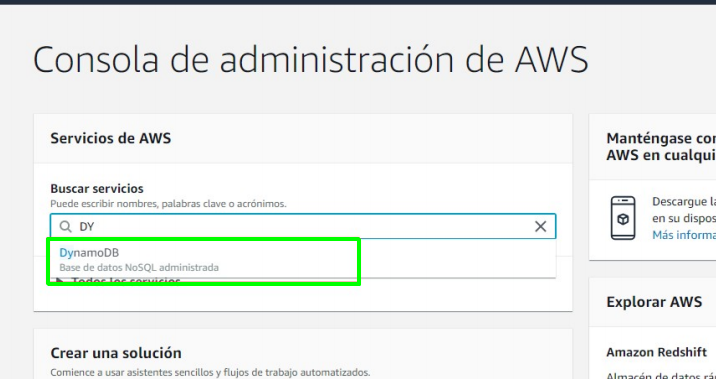
\includegraphics[width=16cm, height=6cm]{img/1.png}\\
		
		\item {Cree un proyecto Aplicación de WPF (.NET Framework) y asignele el nombre SimpleWPFApp. Se abre WPF Designer y se muestra la MainWindow del proyecto.
}\\
		
		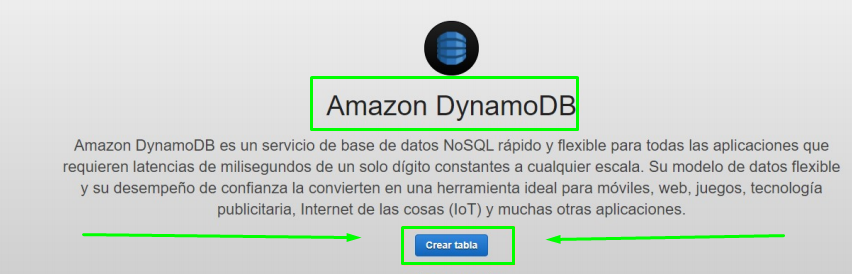
\includegraphics[width=16cm, height=6cm]{img/2.png}\\
	\end{itemize}

	\newpage
	\begin{itemize}
		\item {En este tutorial utilizaremos una biblioteca de musica como nuestro caso de uso. En el campo Table name (Nombre de la tabla), escriba Music.
}\\
		
		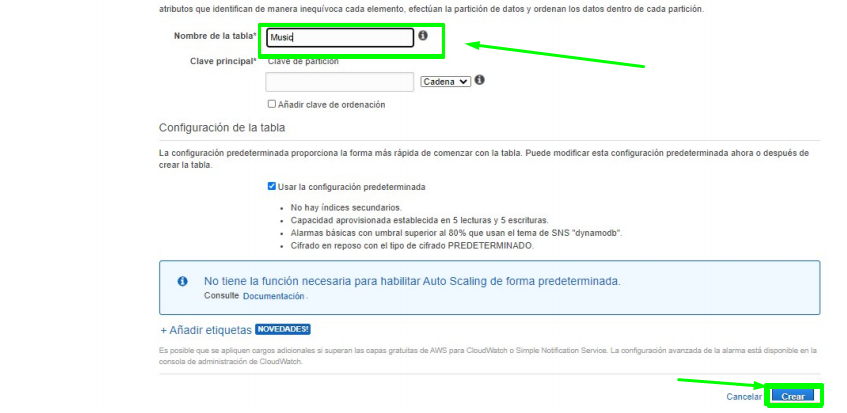
\includegraphics[width=16cm, height=6cm]{img/3.png}\\
		
		\item {La clave de partición se utiliza para repartir datos por las particiones con fines de escalabilidad. Es importante elegir un atributo con una amplia gama de valores y que es probable que tenga patrones de acceso de distribución uniforme. Escriba Artist en el campo Partition Key (Clave de partición).
}\\
		
		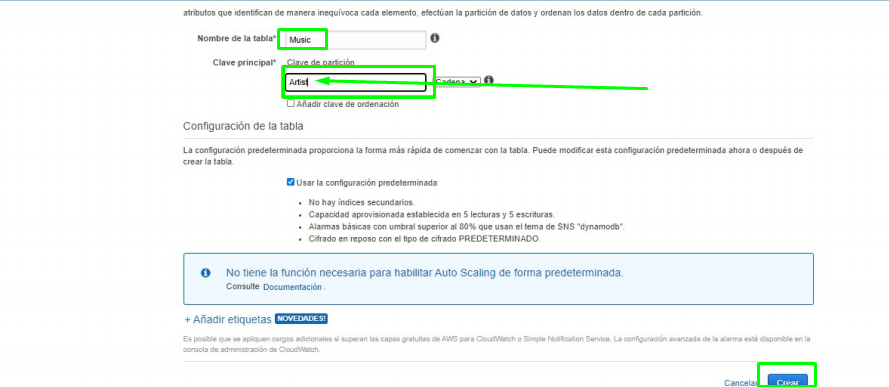
\includegraphics[width=16cm, height=6cm]{img/4.png}\\
		
		\item {Dado que cada artista puede componer muchas canciones, puede habilitar el ordenamiento sencillo con una clave de ordenamiento. Marque la casilla Add sort key (A˜nadir clave de ordenamiento). Escriba songTitle en el campo Add sort key (A˜nadir clave de ordenamiento).
}\\
		
		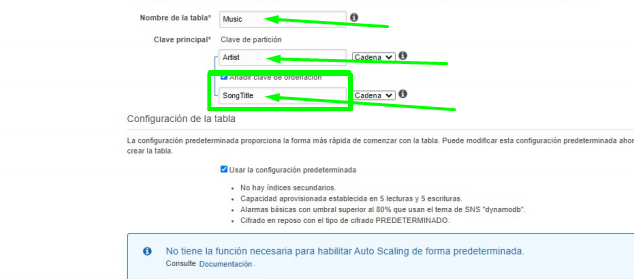
\includegraphics[width=16cm, height=6cm]{img/5.png}\\
		
	\end{itemize}


	\newpage
\begin{itemize}
	\item {A continuacion, activaremos DynamoDB Auto Scaling para nuestra tabla.
		DynamoDB Auto Scaling modificar´a la capacidad de lectura y escritura de su tabla en funcion del volumen de solicitudes. Mediante el uso de una funcion de AWS Identity and Access Management (IAM) denominada DynamoDBAutoscaleRole, DynamoDB administrara el proceso de Auto Scaling por usted. DynamoDB creara esta funcion por usted la primera vez que active Auto Scaling en una cuenta.
		Indique a DynamoDB que cree la funcion mediante la anulacion de la seleccion de Use default settings (Utilizar configuraci´on predeterminada).}\\
	
	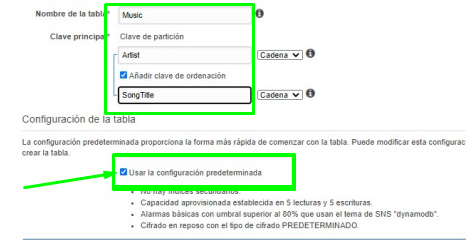
\includegraphics[width=16cm, height=8cm]{img/6.png}\\
	

	
	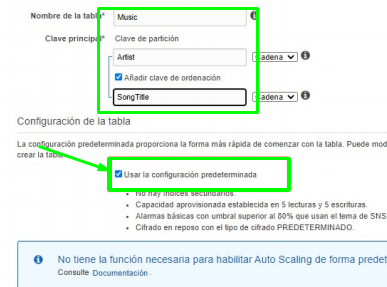
\includegraphics[width=16cm, height=6cm]{img/7.png}\\
	
\end{itemize}



	\newpage
\begin{itemize}
	\item {Desplacese hacia la parte inferior de la pantalla, pasando Secondary indexes (´Indices secundarios), Provisioned capacity (Capacidad aprovisionada) y Auto Scaling hasta llegar al boton Create (Crear). No modificaremos estos par´ametros para los fines de este tutorial.
		
		En la seccion Auto Scaling, observe que DynamoDB crear´a la funci´on DynamoDBAutoscaleRole por usted.
		
		Ahora seleccione Create (Crear).
		
		Cuando la tabla Music este lista para su uso, aparecera en la lista de tablas con una marca de verificacion .
		
		¡Enhorabuena! Acaba de crear una tabla NoSQL con la consola de DynamoDB.}\\
	
	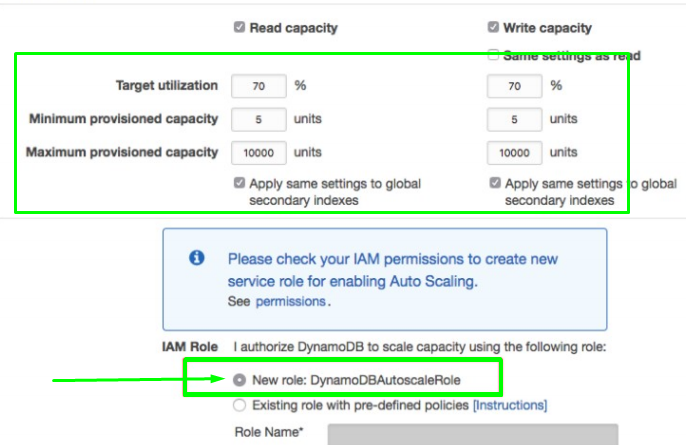
\includegraphics[width=16cm, height=9cm]{img/8.png}\\
	
	
	
	\item {Paso 2: agregar datos a la tabla NoSQL}\\
	
	\item {Haga clic en la pestaña Items (Elementos). Bajo la pestaña Items (Elementos), haga clic en Create item (Crear elemento)}\\
	
	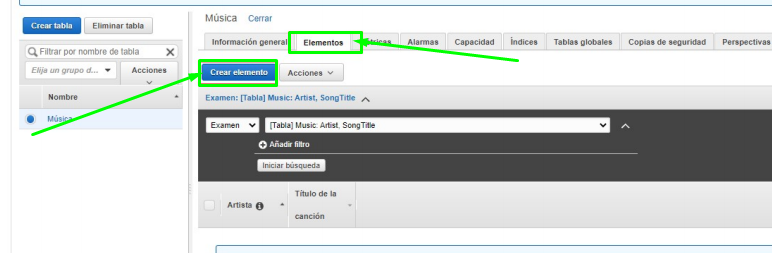
\includegraphics[width=16cm, height=10cm]{img/9.png}\\
	
	\item {En la ventana de introduccion de datos, escriba lo siguiente: Para el atributo Artist, escriba No One You Know. Para el atributo SongTitle , escriba Call Me Today. Haga clic en Save (Guardar) para guardar el elemento.}\\
	
	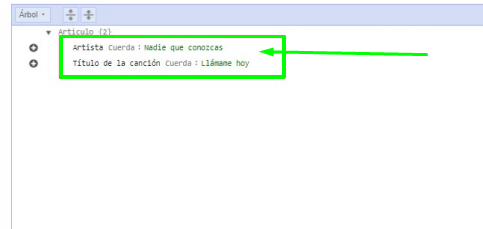
\includegraphics[width=16cm, height=6cm]{img/10.png}\\
	
\end{itemize}

\newpage

\begin{itemize}
	\item {Repita el proceso para agregar algunos elementos mas a la tabla Music:
		Artist: No One You Know; songTitle: My Dog Spot Artist: No One You Know; songTitle: Somewhere Down The Road Artist: The Acme Band; songTitle: Still in Love Artist: The Acme Band; songTitle: Look Out, World}\\
	
	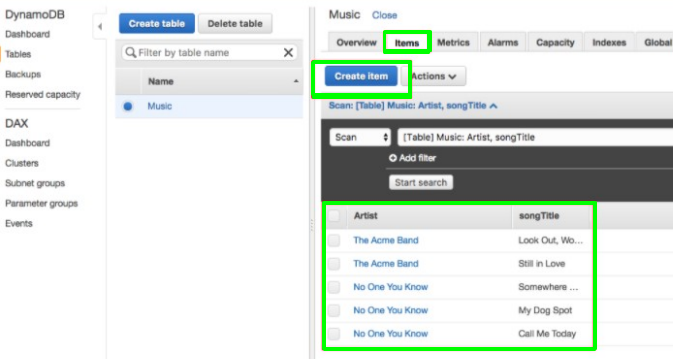
\includegraphics[width=16cm, height=8cm]{img/11.png}\\
	
	\item {Mediante la lista desplegable situada en el banner gris oscuro encima de los elementos, cambie Scan (Escaneo) a Query (Consulta).}\\
	
	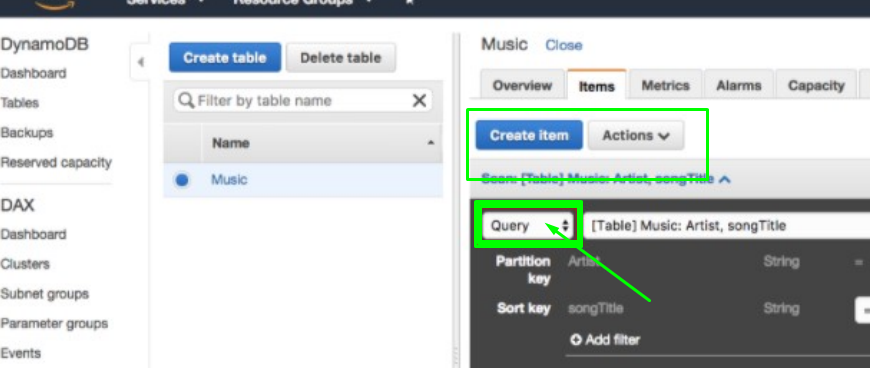
\includegraphics[width=16cm, height=6cm]{img/12.png}\\
	
\end{itemize}

\newpage

\begin{itemize}
	\item {Cree un acceso directo en el escritorio a la aplicacion SimpleWPFApp. Haga clic con el boton derecho en SimpleWPFApp.exe y elija Copiar. En el escritorio, haga clic con el boton derecho y elija Pegar acceso directo. Sugerencia Un acceso directo a la aplicacion facilita el poder agregar o modificar pruebas automatizadas de IU para la aplicacion porque permite iniciar la aplicacion rapidamente}\\
	
	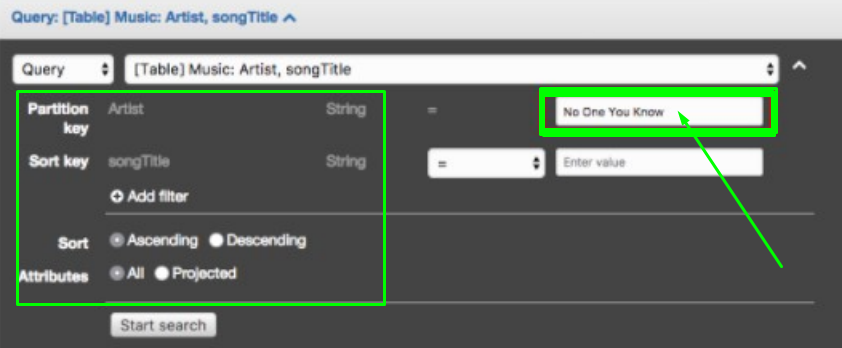
\includegraphics[width=16cm, height=8cm]{img/13.png}\\
	
	\item {Pruebe con otra consulta, pero esta vez acote los resultados de busqueda:
		En el campo Artist, escriba The Acme Band. En el campo SongTitle, seleccione Begins with (Empieza por) en la lista desplegable y escriba S. Haga clic en Start search (Iniciar busqueda). Solo se muestra “Still in Love” interpretada por The Acme Band.
}\\
	
	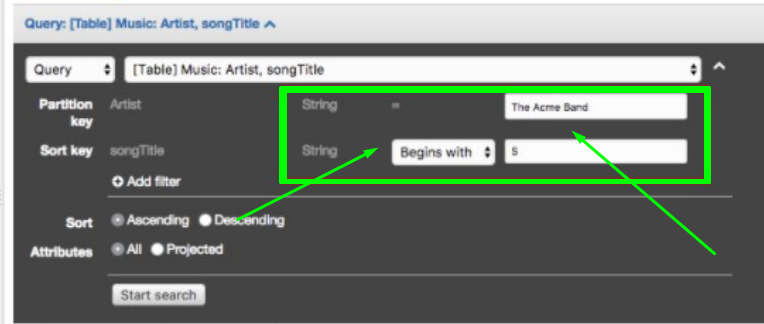
\includegraphics[width=16cm, height=6cm]{img/14.png}\\
	
\end{itemize}


\newpage

\begin{itemize}
	\item {En el Explorador de soluciones, haga clic con el boton derecho en la solucion y elija Agregar ¿Nuevo proyecto
}\\
	
	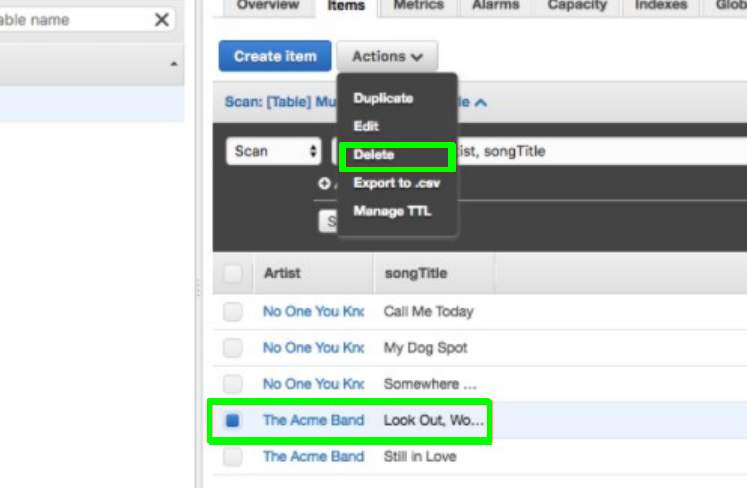
\includegraphics[width=16cm, height=8cm]{img/15.png}\\
	
	\item {Puede eliminar con facilidad una tabla de la consola Amazon DynamoDB. Se recomienda eliminar las tablas que ya no utilice para que no le sigan cobrando por ellas. En la consola de DynamoDB, haga clic en el bot´on de selecci´on ubicado junto a la tabla Music y, a continuaci´on, haga clic en Delete table (Eliminar tabla). En el cuadro de dialogo de confirmacion, haga clic en Delete (Eliminar).}\\
	
	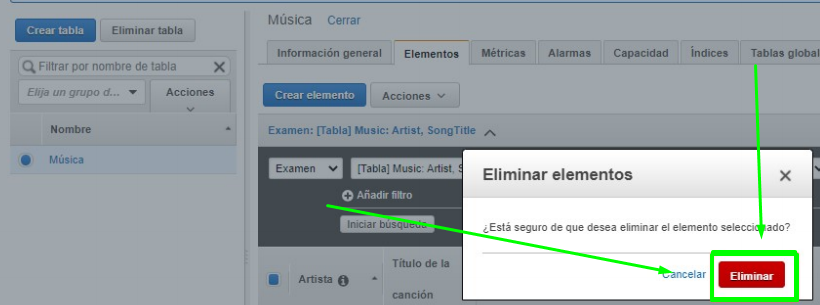
\includegraphics[width=16cm, height=6cm]{img/16.png}\\
	
\end{itemize}

\end{document}